% !TEX root = ../notes.tex

% ================ Data Wrangling ==============
\section{Data Wrangling}

\begin{figure}[H]%---------------FIG--------------
 \centering
 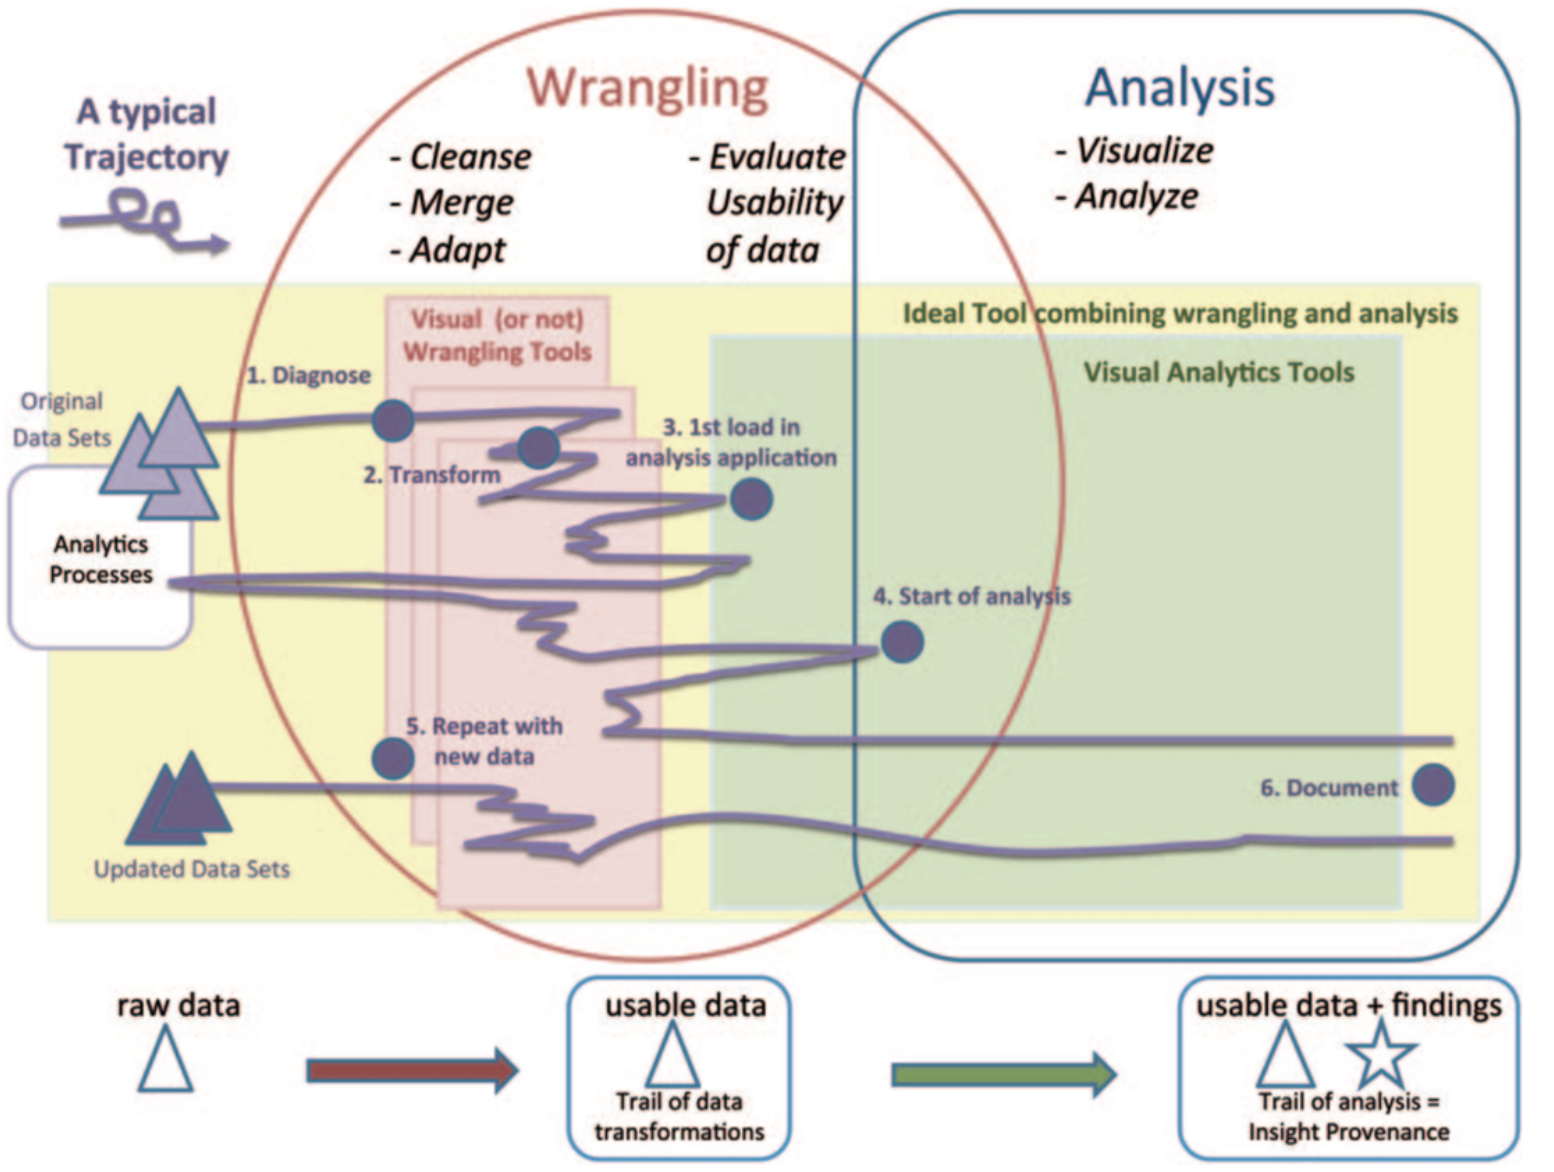
\includegraphics[width=12cm]{./pic/path_data_wrangling}
 \caption{\label{path_data_wrangling}Things do not always happen as expected...}
\end{figure}

Before any analysis, data need to be transformed from "dirty" to clean and processable data. 

Data comes from different sources (excel or SQL?), sometime collected through different methods over time, with different conventions (space or NaN?), etc ... Data wrangling goal is to \textbf{extract and standardize these raw data}. The best way to do it is to \textbf{combine automation with visualizations} in order to find outliers. 

Data problems can come from (non-exhaustive): 
\begin{itemize}
  \item Missing data
  \item Incorrect data
  \item Inconsistent representations of the same data
  \item Non-standardized data (centimeter or inches? Fahrenheit or Celsuis ?)
  \item Duplicated data
\end{itemize}

About 75\% of theses problems will need \textbf{human intervention} to be corrected (by the data-scientist or by crowdsourcing).

Even if it seems really dirty, \textbf{beware not to over-sanitize the data!}. Applying what we can call "defensive programming" is not a good idea because we risk losing any interesting data, keeping only the ones that fit perfectly in our model.

\subsection{Diagnosis of the data}

One of the most important aspects of Data Wrangling is to {\bf understand} the data and to {\bf find possible problems}. In order to ``diagnose'' the data, two tools can be used:
\begin{itemize}
 \item {\bf Visualization} (A {\it thoughtful} visualization will always help)
 \item {\bf Basic Statistics} 
\end{itemize}

Matrix visualizations of the facebook graph is shown in Figure \ref{pic:fb}. The Relational visualization, Figure \ref{pic:fb1}, does not show any particular problem in the data. But the Time dependant visualization, Figure \ref{pic:fb2}, shows that the Facebook API reached its limit while collecting data.

\begin{figure} [h] %----------- SubGraph ---------------------
\centerline{
\subfigure[Relational visualization \label{pic:fb1}] {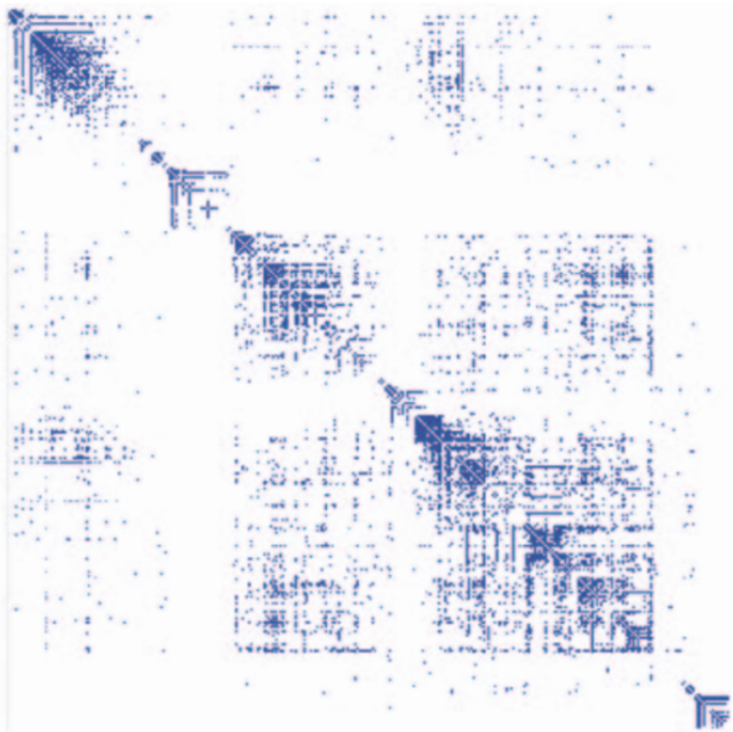
\includegraphics[width=7cm]{pic/fb1} }
\subfigure[Time dependant visualization\label{pic:fb2}] {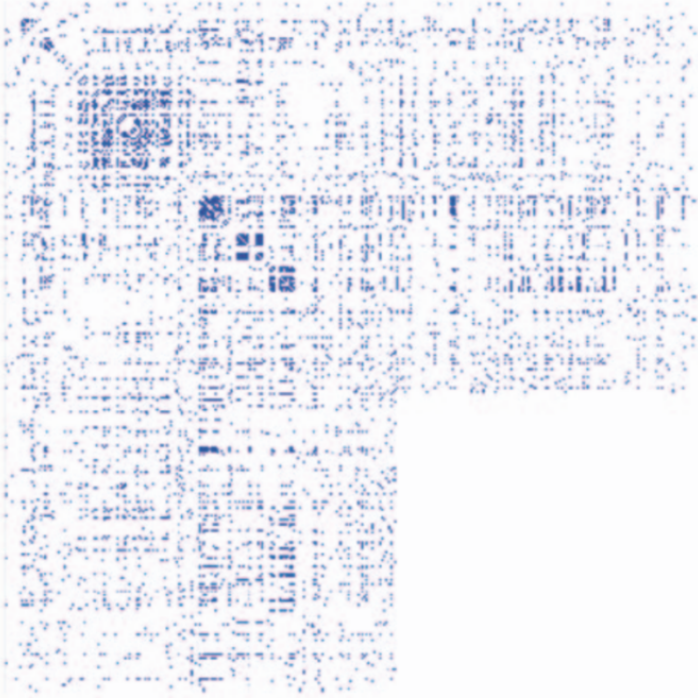
\includegraphics[width=7cm]{pic/fb2} } 
}
\caption{\label{pic:fb} Matrix visualization of the facebook graph.} 
\end{figure}


\subsection{Dealing with missing values}

Values can often miss from the data we have, because of various events (war, fire, ...). We must detect and correct these values with different methods according to the domain we are working in.

Whatever the method used, it's good to keep track of these changes to know which are original data and which are modified ones.

\begin{itemize}
  \item Set values to zero FIG \ref{miss_val}(a)
  \item Interpolate based on existing data FIG \ref{miss_val}(b)
  \item Omit missing data FIG \ref{miss_val}(c)
  \item Interpolation with tracks kept \ref{miss_val}(d)
\end{itemize}

\begin{figure}[H]%---------------FIG--------------
 \centering
 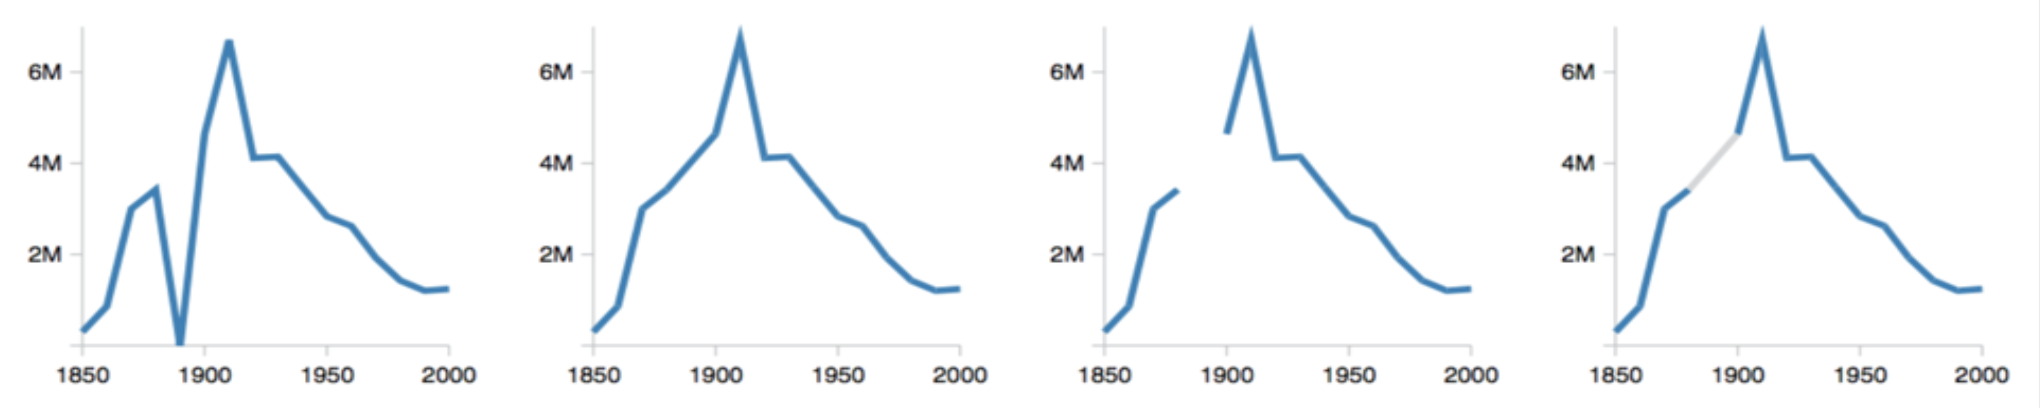
\includegraphics[width=15cm]{./pic/missing_values}
 \caption{\label{miss_val}To deal with missing values.}
\end{figure}

\subsection{General procedure}

Once the data are well wrangled and before trying to analyse them, we must take care of two more steps:

\begin{enumerate}
  \item \textbf{Deal with uncertain data} (can arise from measurement errors, wrong sampling strategies, etc.)
  \item \textbf{Parse/transform data} (with aggregation and reduction techniques) to obtain meaningful records
\end{enumerate}
 
It's always ideal to have the code and/or the documentation about the dataset you are analyzing (provenance).
 